%%%%%%%%%%%%%%%%%%%%%%%%%%%%%%%%%%%%%%%%%
% Friedrich M. Grabner - 01220997
% HPC Coursework
%%%%%%%%%%%%%%%%%%%%%%%%%%%%%%%%%%%%%%%%%

%----------------------------------------------------------------------------------------
%	PACKAGES AND DOCUMENT CONFIGURATIONS
%----------------------------------------------------------------------------------------
\documentclass[10pt, a4paper]{article}
\usepackage{amsmath, amsthm, amssymb}
\usepackage{graphicx} % Required for the inclusion of images
\usepackage{natbib} % Required to change bibliography style to APA
\usepackage{nomencl}
\usepackage{setspace}
\usepackage{geometry} 
\usepackage{hyperref}
\usepackage{subcaption}
\usepackage{xcolor}
\usepackage{lmodern}
\usepackage{listings}
\lstset{language=[90]Fortran,
  basicstyle=\ttfamily,
  keywordstyle=\color{red},
  commentstyle=\color{green},
  morecomment=[l]{!\ }% Comment only with space after !
}

\geometry{a4paper,total={170mm,257mm},left=20mm,top=20mm}



\setlength\parindent{5pt} % Removes all indentation from paragraphs
\graphicspath{{./images/}}
\DeclareGraphicsExtensions{.pdf,.PDF,.jpg,.JPG,.bmp,.png,.eps,.EPS}

%\usepackage{times} % Uncomment to use the Times New Roman font

\input{/home/fmg215/Documents/latex/symbols.tex}
%----------------------------------------------------------------------------------------
%	DOCUMENT INFORMATION
%----------------------------------------------------------------------------------------
\newcommand*{\plogo}{\fbox{$\mathcal{PL}$}}

\newcommand*{\titleGM}{\begingroup % Create the command for including the title page in the document
\hbox{ % Horizontal box
\hspace*{0.2\textwidth} % Whitespace to the left of the title page
\rule{1pt}{\textheight} % Vertical line
\hspace*{0.05\textwidth} % Whitespace between the vertical line and title page text
\parbox[b]{0.75\textwidth}{ % Paragraph box which restricts text to less than the width of the page

{\noindent\huge\bfseries High Performance Computing \\[0.5\baselineskip] AE3-422}\\[2\baselineskip] % Title
{\Large \textsc{F. M. Grabner - 01220997}}\\[4\baselineskip] % Tagline or further description
{\large } % Author name

\vspace{0.5\textheight} % Whitespace between the title block and the publisher
{\noindent Imperial College London - Department of Aeronautics}\\[\baselineskip] % Publisher and logo
}}
\endgroup}
%----------------------------------------------------------------------------------------
%	TITLE PAGE
%----------------------------------------------------------------------------------------
\begin{document}
\titleGM
%----------------------------------------------------------------------------------------
%	QUESTION 1
%----------------------------------------------------------------------------------------
\section*{Question 1}
Matrices have been set up in banded format to minimise the memory utilised. Then the system is solved using Lapack\cite{Lapack1999} function DGBSV. However to leverage the Fortran routines in BLAS\cite{Blas1979}, arrays are in column-major storage format.

Figure \ref{fig:task1} shows the analytical solution against computed solution using the static equations. The computed solution is practically identical to that of the analytical, for the coarse discretisation of 24 elements.

\begin{figure}[!htb]
  \centering
	  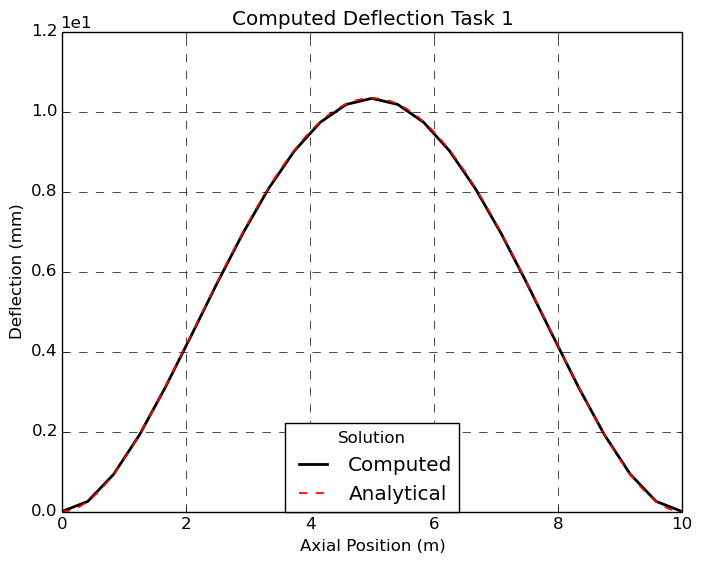
\includegraphics[width=.5\linewidth, clip=true, trim=0cm 0cm 0cm 0cm]{task1}
  \caption{Static against analytical solutions, using $N_x = 24$.}
  \label{fig:task1}
\end{figure}%

%----------------------------------------------------------------------------------------
%	QUESTION 2
%----------------------------------------------------------------------------------------
\section*{Question 2}
Matrix storage identical to task 1. Matrix-vector multiplication has been implemented using BLAS level 3 routine \url{dgbmv}, and then the explicit central-difference scheme is solved using \url{dgbsv}.

\begin{figure}[!htb]
\centering
\begin{subfigure}{.5\textwidth}
  \centering
  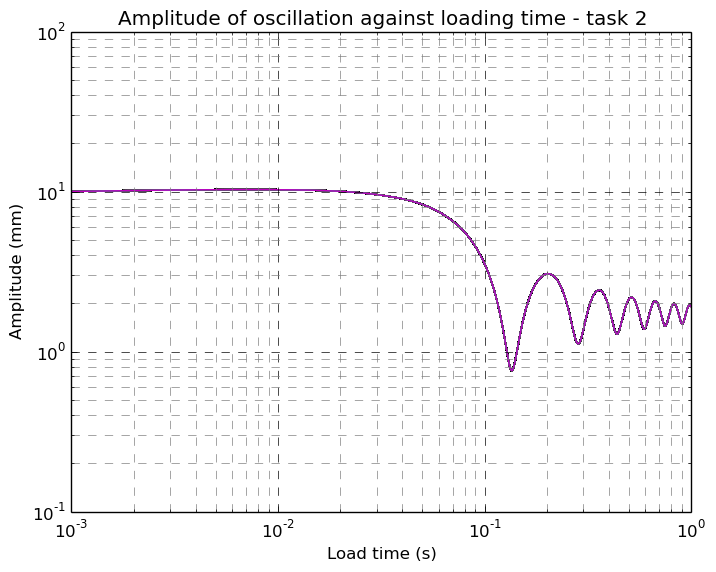
\includegraphics[width=1\linewidth]{task2_amplitude}
  \caption{Amplitude of oscillations.}
  \label{fig:amplitude2}
\end{subfigure}%
\begin{subfigure}{.5\textwidth}
  \centering
  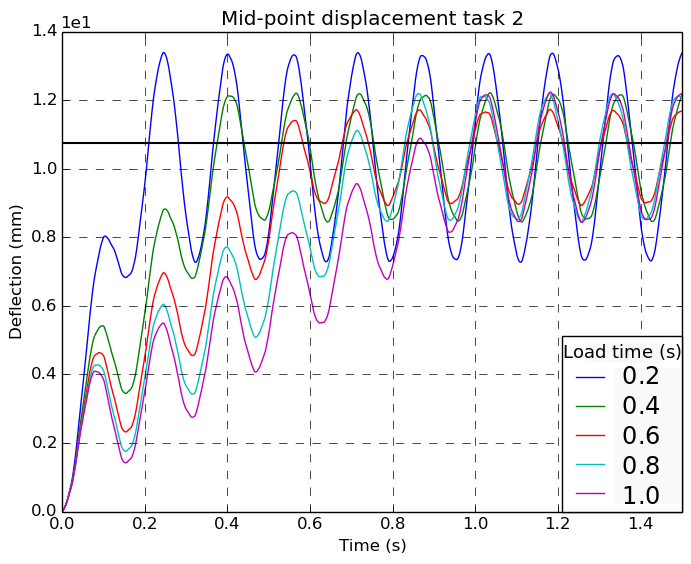
\includegraphics[width=1\linewidth]{task2_deflection}
  \caption{Oscilation with different loading factors.}
  \label{fig:deflection2}
\end{subfigure}
\caption{Grid Independence Test.}
\label{fig:task2}
\end{figure}
\noindent
Figure \ref{fig:deflection2} shows the deflection at beam midpoint against time, for a number of different loading times. In figure \ref{fig:amplitude2} the amplitude of oscillations as the loading time is increased from $0 - 1 (s)$ in steps of size $\Delta t = 0.001 s$ is shown. In general as load time increases, the amplitude of oscillations are seen to decrease. However a number of peaks and troughs exist which are of significantly higher and lower amplitudes. The peaks of amplitude likely correspond to the natural frequency modes of the system, and thus we see that a time of $0.8s$ exhibits lower amplitude oscillations than that of $1s$.
%----------------------------------------------------------------------------------------
%	QUESTION 3
%----------------------------------------------------------------------------------------
\section*{Question 3}
Matrix storage identical to task 1. Matrix-vector multiplications have been implemented using for loops, as the identity matrix can be stored as a vector and using compiler flags \url{-O2} or \url{-O3} produces faster code than the BLAS routine \url{dgbmv} for the diagonal matrix, as the compiler performs some loop-unrolling and the call time is saved. The matrix system was solved using \url{dgbsv}.

\begin{figure}[!htb]
\centering
\begin{subfigure}{.5\textwidth}
  \centering
  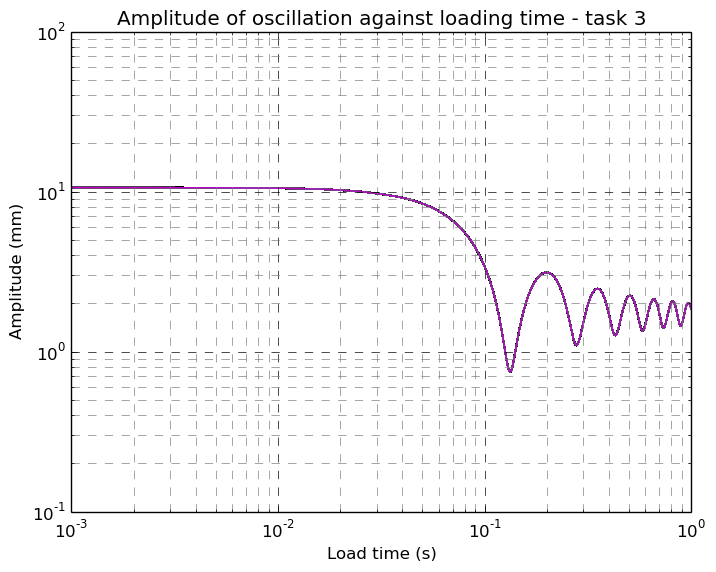
\includegraphics[width=1\linewidth]{task3_amplitude}
  \caption{Amplitude of oscillations.}
  \label{fig:amplitude3}
\end{subfigure}%
\begin{subfigure}{.5\textwidth}
  \centering
  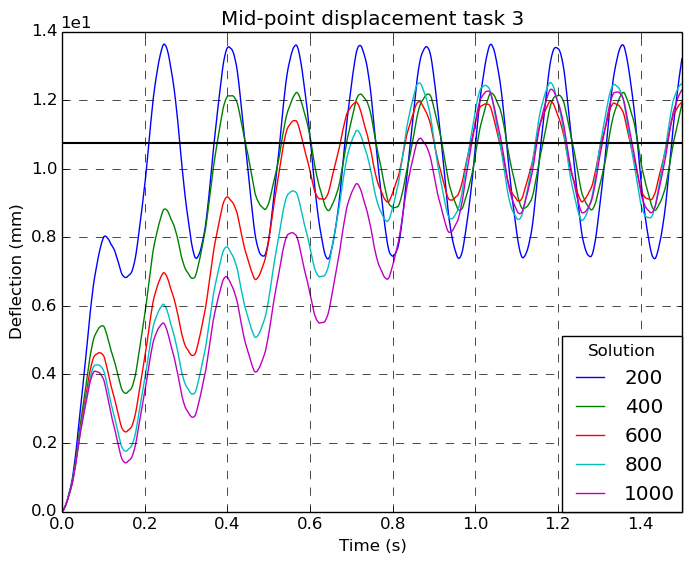
\includegraphics[width=1\linewidth]{task3_deflection}
  \caption{Oscilation with different loading factors.}
  \label{fig:deflection3}
\end{subfigure}
\caption{Grid Independence Test.}
\label{fig:task3}
\end{figure}
\noindent
Using the implicit Newmark scheme the beam exhibits an almost identical response to that of the explicit integration scheme. Again some sort of frequency response is seen in that certain frequencies have significantly lower amplitude than others however the general trend is to an oscillation at order of magnitude $\approx 1mm$. Due to the implicit scheme the solution is found using far fewer timesteps.

%----------------------------------------------------------------------------------------
%	QUESTION 4
%----------------------------------------------------------------------------------------
\section*{Question 4}
Matrix storage as in task 1. In task 4 the beam was solved across multiple processors. Parallel linear algebra solver Scalapack\cite{scalapack1997} was \textbf{not} used. To perform the matrix multiplication BLAS routine \url{dgbmv} was used with an overlap region which allowed contributions to the solution to be accounted for across processes. These contributions were then passed across nodes using MPI\cite{MPI-2.2} at the end of each timestep. The solution was then found simply by inversing the diagonal mass matrix, as this the requires simply multiplication against the right hand side of the equation. However the inverse matrix was stored in an independent array as division is a costly operation,.

\begin{figure}[!htb]
  \centering
	  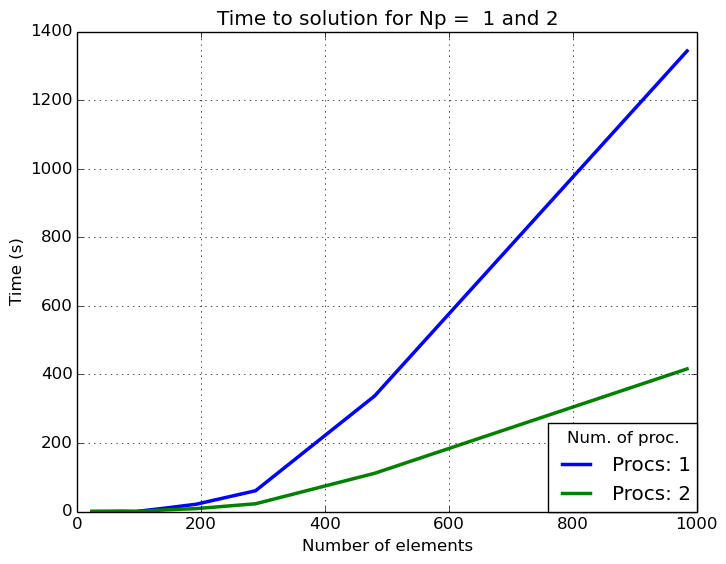
\includegraphics[width=.5\linewidth, clip=true, trim=0cm 0cm 0cm 0cm]{task4_timing}
  \caption{Time to solution as problem size increases with 1 and 2 processors.}
  \label{fig:timing4}
\end{figure}%
\noindent
Above in figure\ref{fig:timing4} the time to solution for different problem sizes is displayed. Clear to see that, except for small problems of less than 200 elements, the MPI routines are significantly quicker. The strong scaling is not seen to be linear, this is due to the problem size not being kept uniform. The decision was taken not to spend too long finding the minimum timesteps to keep the larger simulations stable and rather to simply match increase in $N_t$ with increases of $N_t$.
%----------------------------------------------------------------------------------------
%	QUESTION 5
%----------------------------------------------------------------------------------------
\section*{Question 5}
Matrix storage in banded as always, however with a buffer of zeros on top for use with Scalapack. Task 5 splits the Newmark method across 1, 2, and 4 processors. This problem allowed use of Scalapacks \url{pdgbsv} routine. Implementing this requires equal block sizes across processes. However the definition of the problem makes this difficult, in order to leverage Scalapack all ranks were filled except the last rank which received any left-over nodes. Then the end zone is padded with zeros and 1s across the diagonal for matrices, filling simply with 0s for vectors. This meant the system was solved easily allowing Scalapack to perform communication. inal points could be discarded.

\begin{figure}[!htb]
  \centering
	  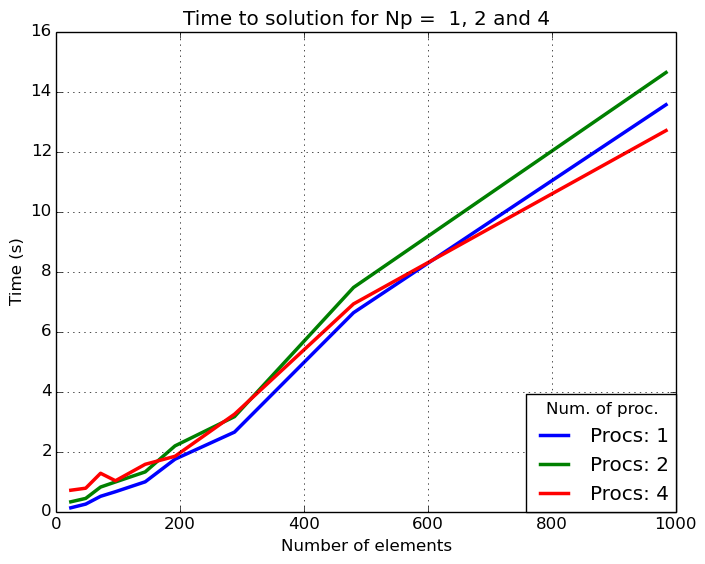
\includegraphics[width=.5\linewidth, clip=true, trim=0cm 0cm 0cm 0cm]{task5_timing}
  \caption{Time to solution as problem size increases with 1, 2 and 4 processors.}
  \label{fig:timing5}
\end{figure}%
\noindent
Figure \ref{fig:timing5} shows the time to solution for 1,2 and 4 processors. For this implicit scheme the timesteps were kept constant at $N_t = 10,000$ for all sizes of $N_x$. The parallel programs only begin to become faster as $N_x >> 500$. This indicates that whilst scalapack efficiently hides communication in the Blacs sublayer, communication takes a large chunk out of the performance, in comparison to serial BLAS routines. However as the problem becomes larger this effect reduces.

%---------------------------------------------------------------------------------------
%	BIBLIOGRAPHY
% ---------------------------------------------------------------------------------------
\bibliographystyle{unsrt}	% in order of appearance
%\bibliographystyle{acm}	% (uses file "plain.bst")
%\bibliographystyle{abbrv}	% (uses file "plain.bst")
%\bibliographystyle{siam}	% (uses file "plain.bst")
%\bibliographystyle{apalike}
\bibliography{/home/fmg215/Documents/latex/myrefs}		% expects file "myrefs.bib"}
%----------------------------------------------------------------------------------------
% END DOCUMENT
%----------------------------------------------------------------------------------------
\end{document}